% --- CHUNK_METADATA_START ---
% src_checksum: 84eb0c2df5d3c0c4da6e792afa5e56e4e9c0a6fdac689895a4dec6100eab3c6e
% needs_review: True
% --- CHUNK_METADATA_END ---
\chapter{Poisson Process}% --- CHUNK_METADATA_START ---
% src_checksum: 72866aa510b3cc88f678364c0035ffe135e58e0d2ca75a0b2e5a6cc256da9ebb
% --- CHUNK_METADATA_END ---
\sloppy% --- CHUNK_METADATA_START ---
% src_checksum: 5002441a02d1aaca20e9459cb1000cc52f358bdc88c40b6295b26fedd14df548
% needs_review: True
% --- CHUNK_METADATA_END ---
\section{Introduction and Motivation}% --- CHUNK_METADATA_START ---
% src_checksum: 72657e0db46c87dcf2368183c18aa071794358e8b4c97fd7f684eebc7054ca34
% needs_review: True
% --- CHUNK_METADATA_END ---
We want to model events that occur at precise but unpredictable dates.% --- CHUNK_METADATA_START ---
% src_checksum: 1d5093b5a2394fc3c631b0ca291fe660aa4bedc2dc281ff40e2446aada68e3ed
% needs_review: True
% --- CHUNK_METADATA_END ---
\begin{example}
Examples of such events include earthquakes, atomic decay, rain, or the beginning and end of telephone calls.
\end{example}% --- CHUNK_METADATA_START ---
% src_checksum: 16a7041434211e294258bd18a2375d5edb1b88dc2de795f7995f2fbfe78b346e
% needs_review: True
% --- CHUNK_METADATA_END ---
At each occurrence of an event, we mark an impact on the time axis.% --- CHUNK_METADATA_START ---
% src_checksum: 1cdab132737f5dc041c4a89aa7118369f058ec0f9f5b5d7d056b0dbab2187180
% --- CHUNK_METADATA_END ---
\begin{figure}[H]
\centering
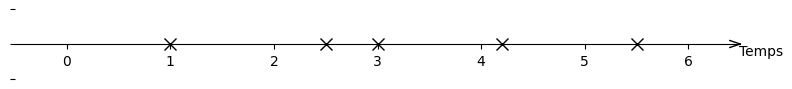
\includegraphics[width=0.8\textwidth]{time_axis_impacts.png}
\end{figure}% --- CHUNK_METADATA_START ---
% src_checksum: cad0eb514e2f45f265db397b164eb31bba9bca6f063a9e95a5a01a2fc6ca1988
% needs_review: True
% --- CHUNK_METADATA_END ---
\section{Model hypotheses}% --- CHUNK_METADATA_START ---
% src_checksum: d551726022daa8074d0ba3394fcd6bfe410eebc64cfdcb54dd67c820aa7a845c
% needs_review: True
% --- CHUNK_METADATA_END ---
To construct our model, we make the following assumptions:% --- CHUNK_METADATA_START ---
% src_checksum: 6788f148f70a4398f2b35cd3001d9e14ed0503b7f3fe5a16b71d5df12899d70a
% needs_review: True
% --- CHUNK_METADATA_END ---
\begin{itemize}
    \item[i)] The experimental conditions do not change over time.
    \item[ii)] The number of impacts in disjoint time intervals is independent.
\end{itemize}% --- CHUNK_METADATA_START ---
% src_checksum: 832a42bf3dd97c5fe17125d29d244980acf294fce86957a9648f116ed0471449
% needs_review: True
% --- CHUNK_METADATA_END ---
For $t \ge 0$, we denote $N(t)$ the number of occurrences in the interval $[0, t]$.
We thus have a family of random variables $(N(t))_{t \ge 0}$ indexed by a continuous parameter. This is a \textbf{stochastic process}.% --- CHUNK_METADATA_START ---
% src_checksum: c05a2b83eedf39090fb8937cff1cc8bb017ef6bcd81fa3b66f3198ecbb1c6f4d
% needs_review: True
% --- CHUNK_METADATA_END ---
\section{Construction of a discrete model}% --- CHUNK_METADATA_START ---
% src_checksum: 59edc1acb69b9f66e94977cf531c9ea0a3780da65ce59d08379735f3b084caf9
% needs_review: True
% --- CHUNK_METADATA_END ---
Let $n \ge 1$ be an integer. We subdivide the real axis into intervals of length $\frac{1}{n}$, of the form $\left[\frac{k}{n}, \frac{k+1}{n}\right[$, for $k \ge 0$.% --- CHUNK_METADATA_START ---
% src_checksum: f72d17e0d6d81f839d905efb3ef5e82f3bbd7bd1f0d8d9cca0e77b203f405aa6
% --- CHUNK_METADATA_END ---
\begin{figure}[H]
\centering
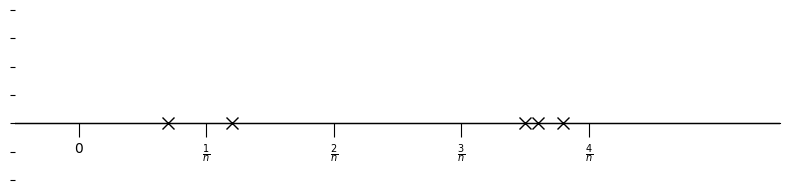
\includegraphics[width=0.8\textwidth]{discrete_time_axis.png}
\end{figure}% --- CHUNK_METADATA_START ---
% src_checksum: 3d79857f2f2fbb8152732f758b32e65755f899dde8c7750b6601cefeb99f6245
% needs_review: True
% --- CHUNK_METADATA_END ---
A range can have $0, 1, 2, \dots$ impacts.% --- CHUNK_METADATA_START ---
% src_checksum: 408313d348592e1ba908557086b5e23c8b908d4cf7462e60e85aa24c9d665ca5
% needs_review: True
% --- CHUNK_METADATA_END ---
\begin{definition}
An interval $\left[\frac{k}{n}, \frac{k+1}{n}\right[$ is called \textbf{occupied} if it contains at least one hit, and \textbf{empty} otherwise.
\end{definition}% --- CHUNK_METADATA_START ---
% src_checksum: 36f6ca99c0fc63830060abc4a3078f48380b40e3c33ff8369fbd2ef956b30fe6
% needs_review: True
% --- CHUNK_METADATA_END ---
Let $p_n$ denote the probability that an interval $\left[\frac{k}{n}, \frac{k+1}{n}\right[$ is occupied. \\
According to hypothesis (i), $p_n$ does not depend on the interval.\\
For $t>0$, let $N_n(t)$ be the number of intervals $\left[\frac{k}{n}, \frac{k+1}{n}\right[$ (with $\frac{k+1}{n} \le t$) that are occupied.\\
By hypothesis (ii), the states (empty or occupied) of these intervals are independent, and $N_n(t)$ follows the binomial distribution $B(\lfloor nt \rfloor, p_n)$.% --- CHUNK_METADATA_START ---
% src_checksum: da435127b9bab131167f252687b7089863d4f14565a2aa165b91a19ef44ee89d
% needs_review: True
% --- CHUNK_METADATA_END ---
\section{Convergence to the Poisson distribution}% --- CHUNK_METADATA_START ---
% src_checksum: 93c6c521229536eca7245e166a9ae20fe84b7f949d0c2c1fc5f72e0be1e97d96
% needs_review: True
% --- CHUNK_METADATA_END ---
We study the limit in distribution of $N_n(t)$, for example using characteristic functions.
The characteristic function of $N_n(t)$ is:
\[ \varphi_{N_n(t)}(u) = E[e^{iu N_n(t)}] = (1 - p_n + p_n e^{iu})^{\lfloor nt \rfloor} \]
We add an additional assumption: $p_n \to 0$ when $n \to \infty$. Otherwise, the model "explodes".
To study the limit, we analyze the logarithm of the characteristic function:% --- CHUNK_METADATA_START ---
% src_checksum: 475033a8e079ea648b5d2a2c5ae75ebd11b45dafde9964d932997c4339d391cf
% --- CHUNK_METADATA_END ---
\begin{align*}
\ln(\varphi_{N_n(t)}(u)) &= \lfloor nt \rfloor \ln(1 - p_n + p_n e^{iu}) \\
&= \lfloor nt \rfloor \ln(1 + p_n(e^{iu} - 1))
\end{align*}% --- CHUNK_METADATA_START ---
% src_checksum: aaa31494b267e78b98607d47573992514db8073b6a76b4cfc7b72985d230ce98
% needs_review: True
% --- CHUNK_METADATA_END ---
By using the limited expansion $\ln(1+x) = x + o(x)$ for $x \to 0$, we obtain:% --- CHUNK_METADATA_START ---
% src_checksum: 002051d722fe344ce73de231bb8187472c07033bae8ea055a44c4073fb9c30cc
% --- CHUNK_METADATA_END ---
\begin{align*}
\ln(\varphi_{N_n(t)}(u)) &= \lfloor nt \rfloor \left( p_n(e^{iu}-1) + o(p_n) \right) \\
&= \lfloor nt \rfloor p_n (e^{iu}-1) + o(n p_n)
\end{align*}% --- CHUNK_METADATA_START ---
% src_checksum: 3bcd93151dbe353e40367745d6156a2e76864dba4ea279fcb548154474b1631c
% needs_review: True
% --- CHUNK_METADATA_END ---
By transitioning to the exponential form:
\[ \varphi_{N_n(t)}(u) = e^{\lfloor nt \rfloor p_n (e^{iu}-1) + o(n p_n)} \]
Assume that $np_n \to \lambda$ as $n \to \infty$, where $\lambda$ is a positive constant. Then $\lfloor nt \rfloor p_n \approx nt p_n \to \lambda t$.
The limit of the characteristic function becomes:
\[ \lim_{n \to \infty} \varphi_{N_n(t)}(u) = e^{\lambda t (e^{iu}-1)} \]
We recognize the characteristic function of a Poisson distribution with parameter $\lambda t$.
Thus, $N_n(t)$ converges in law to a random variable following a Poisson distribution $\mathcal{P}(\lambda t)$.
\[ N_n(t) \xrightarrow{\mathcal{L}} \mathcal{P}(\lambda t) \]% --- CHUNK_METADATA_START ---
% src_checksum: 0e6e81fee2417b4645e9a68aaf4eefb04482750243c5281f7f8327cd09659efb
% needs_review: True
% --- CHUNK_METADATA_END ---
\begin{remark}[Reminder on the Poisson Distribution]
A random variable $X$ taking values in $\mathbb{N}$ follows a Poisson distribution with parameter $\lambda > 0$, denoted $X \sim \mathcal{P}(\lambda)$, if for all $k \in \mathbb{N}$:
\[ P(X=k) = e^{-\lambda} \frac{\lambda^k}{k!} \]
Its \textbf{expectation} and its \textbf{variance} are equal to $\lambda$, i.e., $E[X] = \text{Var}[X] = \lambda$.\\
Its \textbf{characteristic function} is $\varphi_X(u) = \exp(\lambda(e^{iu}-1))$.
\end{remark}% --- CHUNK_METADATA_START ---
% src_checksum: 9d5ee24db21fe5904389c6da2ce66a106c1a89ddec436a732b1d988faa32407e
% needs_review: True
% --- CHUNK_METADATA_END ---
\section{Jump Instants}% --- CHUNK_METADATA_START ---
% src_checksum: c324c213ff43268b27c09f64dcb938a92c908f9d1196f4797df39bfdd9d5af3a
% needs_review: True
% --- CHUNK_METADATA_END ---
We have shown that, at fixed $t$, $N_n(t) \xrightarrow{\mathcal{L}} \mathcal{P}(\lambda t)$.
However, the function $t \mapsto N_n(t)$ is a \textbf{random step function}, which is zero at 0, increasing, and whose increments are either 0 or 1.% --- CHUNK_METADATA_START ---
% src_checksum: f458d03f0bd56026c481b59959b7f213b2028941fa7ef75b6f0844620ce57a8b
% needs_review: True
% --- CHUNK_METADATA_END ---
\begin{figure}[H]
\centering
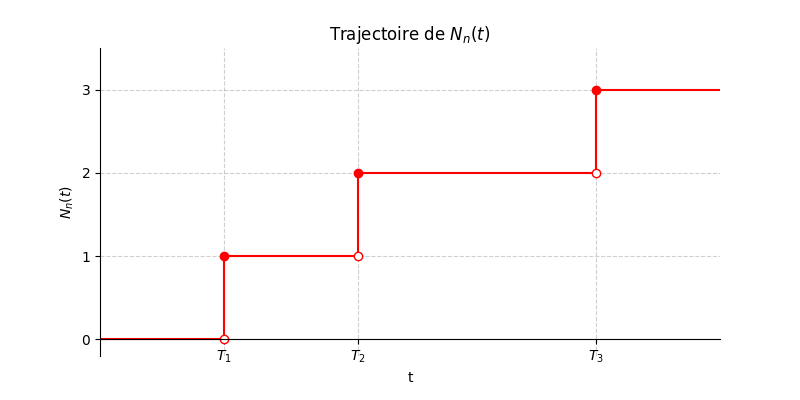
\includegraphics[width=0.8\textwidth]{Nn_t_plot.png}
\caption{A realization of the random function $t \mapsto N_n(t)$.}
\end{figure}% --- CHUNK_METADATA_START ---
% src_checksum: 3141a81abbe023f45fd87c7bfb13b205ab374f2df3b7ef5f76c8ea959278079e
% needs_review: True
% --- CHUNK_METADATA_END ---
The question arises: does the random function $t \mapsto N_n(t)$ converge when $n \to \infty$?
The function $N_n(t)$ is completely determined by its jump times. We define the jump times of $N_n(t)$ as:
\[ \forall k \ge 1, \quad T_k^n = \inf\left\{t \ge 0 : N_n(t)=k\right\} \]
Indeed, we have $N_n(t) = \sum_{k=1}^\infty 1_{\{T_k^n \le t\}}$.
Let us examine the convergence of these jump times, starting with $T_1^n$.
Let $i \ge 0$ be an integer. The event $\{T_1^n > i/n\}$ means that the first $i$ time intervals, $[0, 1/n), [1/n, 2/n), \dots, [(i-1)/n, i/n)$,% --- CHUNK_METADATA_START ---
% src_checksum: 4a5d7bf8d2ad34a7071874cc7ce2d913981d9e49da303064b88d12f99d2fa80a
% needs_review: True
% --- CHUNK_METADATA_END ---
, are all empty.
To analyze this, we introduce a sequence of random variables $X_k$ for $k \ge 0$:
\[ X_k = \begin{cases} 0 & \text{si l'intervalle } [k/n, (k+1)/n[ \text{ est vide} \\ 1 & \text{sinon (occupé)} \end{cases} \]
Then $P(T_1^n > i/n) = P(X_0=0, \dots, X_{i-1}=0)$. By independence, this equals $(1-p_n)^i$.
For a fixed $t>0$, let us choose $i = \lfloor nt \rfloor$. Then:
\[ P(T_1^n > t) \approx P(T_1^n > \lfloor nt \rfloor / n) = (1-p_n)^{\lfloor nt \rfloor} \]
Since we assumed $np_n \to \lambda$, we have $p_n \approx \lambda/n$.
\[ P(T_1^n > t) \approx \left(1-\frac{\lambda}{n}\right)^{nt} \xrightarrow[n\to\infty]{} e^{-\lambda t} \]% --- CHUNK_METADATA_START ---
% src_checksum: 8acbb02b364867ab2144c1333ceb6dba9322b9fb4d4e3c293a80dad4cfae41c7
% needs_review: True
% --- CHUNK_METADATA_END ---
We recognize the survival function of an exponential distribution. Therefore, $T_1^n \xrightarrow{\mathcal{L}} \text{Exp}(\lambda)$.% --- CHUNK_METADATA_START ---
% src_checksum: f1c89a7ef0c39df04b735340b4a04068555a28092a87b83e24bb49a35c45c95e
% needs_review: True
% --- CHUNK_METADATA_END ---
\begin{remark}[Reminder on the Exponential Distribution]
A random variable $X$ follows the exponential distribution with parameter $\lambda > 0$, denoted $\text{Exp}(\lambda)$, if its density function is $f(x) = \lambda e^{-\lambda x}$ for $x \ge 0$.
Its expectation is $E[X] = 1/\lambda$ and its variance is $\text{Var}[X] = 1/\lambda^2$.
Its cumulative distribution function is $F_X(x) = P(X \le x) = 1 - e^{-\lambda x}$ for $x \ge 0$.
\end{remark}% --- CHUNK_METADATA_START ---
% src_checksum: 11290ecc696241535f56adb18fcfd54706969d91eb8f8786a7fff9dd0a8a0692
% needs_review: True
% --- CHUNK_METADATA_END ---
\begin{figure}[H]
    \centering
    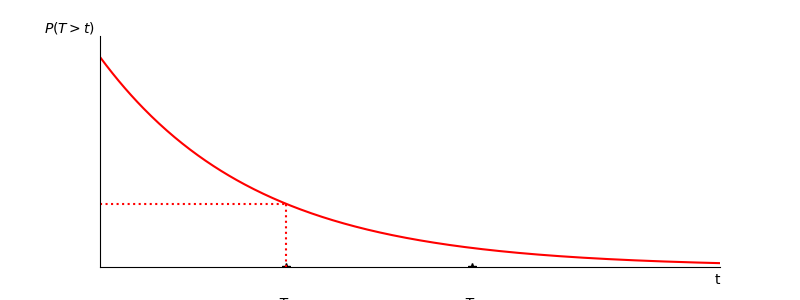
\includegraphics[width=0.7\textwidth]{exp_survival.png}
    \caption{Survival function of the exponential distribution.}
\end{figure}% --- CHUNK_METADATA_START ---
% src_checksum: fa87fdee2896bbdba147f2c287d0ad4dfe817df543f9bda762db59e20a686d59
% needs_review: True
% --- CHUNK_METADATA_END ---
Furthermore, it can be shown that the durations between successive jumps are independent and identically distributed. For example, $T_2^n - T_1^n$ is independent of $T_1^n$ and also converges in distribution to $\text{Exp}(\lambda)$. Let us verify this for the discrete model.% --- CHUNK_METADATA_START ---
% src_checksum: 83f903277120cc8b012b7785eea8632a86ffd38b7f0ea11868cd3612b366ea06
% needs_review: True
% --- CHUNK_METADATA_END ---
\begin{remark}
Let $i,j \ge 1$.\\
$$P(T_1^n = i/n, T_2^n - T_1^n = j/n) = P(X_0=0, \dots, X_{i-1}=0, X_i=1, X_{i+1}=0, \dots, X_{i+j-1}=0, X_{i+j}=1)$$.
This probability equals $(1-p_n)^{i-1} p_n \cdot (1-p_n)^{j-1} p_n$.
This is equal to $P(T_1^n = i/n) \cdot P(T_1^n = j/n)$. Hence the result.\\
Thus, the inter-jump vector converges in distribution:
\[ (T_1^n, T_2^n - T_1^n, \dots, T_k^n - T_{k-1}^n) \xrightarrow[n\to\infty]{\mathcal{L}} (\text{Exp}(\lambda))^{\otimes k} \]
that is, toward a vector of $k$ independent and identically distributed random variables with distribution $\text{Exp}(\lambda)$.
\end{remark}% --- CHUNK_METADATA_START ---
% src_checksum: 75e14738d470dca0d2084319d021a9d93fecd833678bb057bf98a5149e81887b
% needs_review: True
% --- CHUNK_METADATA_END ---
\section{The Continuous Poisson Process}% --- CHUNK_METADATA_START ---
% src_checksum: 23bfc6910a1728f1ae2840cedebac28c8d97f250a32eb729d52002ab24339fa6
% needs_review: True
% --- CHUNK_METADATA_END ---
The previous calculations allow us to envision the candidate for the limit in law of $N_n(t)$.% --- CHUNK_METADATA_START ---
% src_checksum: d3b0c9575ac8bbdb5789042c2a83b4bd8ad30507a52f04e75446ce77fcfa63b3
% needs_review: True
% --- CHUNK_METADATA_END ---
\subsection{Definition from jump moments}% --- CHUNK_METADATA_START ---
% src_checksum: 5af259655ef7a6a8a7a2724f2fb7dba5aa88329857c9f44c0f1aae4e875069b6
% needs_review: True
% --- CHUNK_METADATA_END ---
Let $(Y_n)_{n \ge 1}$ be a sequence of independent and identically distributed random variables following the exponential distribution $\text{Exp}(\lambda)$.
Let $S_0=0$ and for $n \ge 1$, $S_n = Y_1 + Y_2 + \dots + Y_n$.
The variable $S_n$ represents the time of the $n$-th event.% --- CHUNK_METADATA_START ---
% src_checksum: 47fe100fac2d53bd970da0b10261db371ddd0739578c96efea2e34ee1e368267
% needs_review: True
% --- CHUNK_METADATA_END ---
\begin{definition}[Poisson Process]
For any $t \ge 0$, we define the number of events up to time $t$ as:
\[ N(t) = \max \{ n \ge 0 : S_n \le t \} \]
The stochastic process $(N(t))_{t \ge 0}$ is called the \textbf{Poisson process} with intensity $\lambda$.
\end{definition}% --- CHUNK_METADATA_START ---
% src_checksum: 87a34389fab850b3b6886c01abd6ea8001ad1aeead3d3dfcad7bbe81ca3a4bea
% --- CHUNK_METADATA_END ---
\begin{figure}[H]
    \centering
    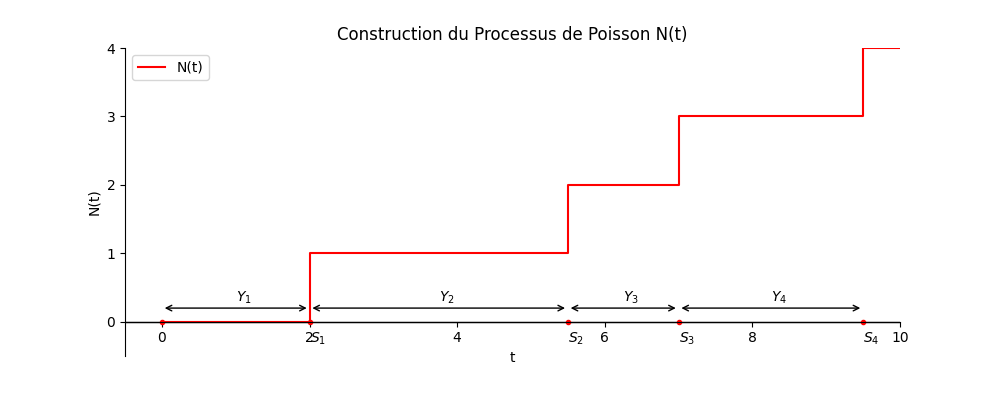
\includegraphics[width=\textwidth, keepaspectratio]{poisson_process_construction.png}
\end{figure}% --- CHUNK_METADATA_START ---
% src_checksum: 4f4d3f7b4e48e5ba260d7ff42be016fc173091ffb069758c2891d0ef3cea3421
% needs_review: True
% --- CHUNK_METADATA_END ---
For each $t$, $N(t)$ is a random variable that follows a Poisson distribution $\mathcal{P}(\lambda t)$.
We have thus constructed a continuum of random variables $(N(t))_{t \ge 0}$ on the same probability space.
We have $S_n \to +\infty$ almost surely. $N(t)$ is the unique index $k$ such that $S_k \le t < S_{k+1}$.% --- CHUNK_METADATA_START ---
% src_checksum: a841cde02432f320ab0e41cc86b9fa808f296d79492b87de162e443de9e21671
% needs_review: True
% --- CHUNK_METADATA_END ---
\section{Applications}% --- CHUNK_METADATA_START ---
% src_checksum: 2e3074a03eddc769ce196cdb9c5eb9e101f6c8014714fbdf3cd0ad548c08e57d
% needs_review: True
% --- CHUNK_METADATA_END ---
\subsection{Application 1: Bombardment of London (WWII)}% --- CHUNK_METADATA_START ---
% src_checksum: 3e1181733d8e981c051eeaf88655e264b7bb0b94991d0eb66603de4ea2cbbe91
% needs_review: True
% --- CHUNK_METADATA_END ---
During World War II, the city of London suffered 537 bomb impacts. The map of the city was divided into a grid of 576 squares of 0.25 km$^2$ each. The average number of impacts per square is therefore $\lambda = 537/576 \approx 0.9323$.
We compare the number of squares receiving $k$ impacts with the predictions of the Poisson distribution $\mathcal{P}(0.9323)$.% --- CHUNK_METADATA_START ---
% src_checksum: ecd2446fdcb5b70419c3fc5fdd77f5a55bdea25d9bd66d2eb2dd0e836ba3b467
% needs_review: True
% --- CHUNK_METADATA_END ---
\begin{figure}[H]
    \centering
    
\includegraphics[width=0.4\textwidth]{london_grid.png}
    \caption{Grid of the London map.}
\end{figure}% --- CHUNK_METADATA_START ---
% src_checksum: e6572e6cee9884944af56245fb3d84d3b9f957cdc801591bbace1bd1b17bd3c5
% needs_review: True
% --- CHUNK_METADATA_END ---
The following table compares the observed data (number of squares with $k$ impacts) and the expected values according to the Poisson distribution ($576 \times P(X=k)$ with $X \sim \mathcal{P}(0.9323)$).% --- CHUNK_METADATA_START ---
% src_checksum: 003a77775353ff2d70d283267e0500c80f106f0f0837484b65d3f86cfa42254c
% needs_review: True
% --- CHUNK_METADATA_END ---
\begin{center}
\begin{tabular}{|c|cccccc|}
\hline
\textbf{k (impacts)} & \textbf{0} & \textbf{1} & \textbf{2} & \textbf{3} & \textbf{4} & \textbf{$\ge 5$} \\
\hline
\textbf{Observed} & 229 & 211 & 93 & 35 & 7 & 1 \\
\textbf{Expected} & 226.74 & 211.39 & 98.54 & 30.62 & 7.14 & 1.57 \\
\hline
\end{tabular}
\end{center}% --- CHUNK_METADATA_START ---
% src_checksum: b28cfa9cb2e35fe40a8868b18da11ffcbb99e595e5ce5f953d8326aa1c19f9a6
% needs_review: True
% --- CHUNK_METADATA_END ---
\subsection{Application 2: Bus Problem}% --- CHUNK_METADATA_START ---
% src_checksum: 3e4b537ab95003bfce190f4e45f364188b177197b0bc6867b8ec6643ae80d44d
% needs_review: True
% --- CHUNK_METADATA_END ---
Bus arrivals at a stop are modeled by a Poisson process with intensity $\lambda$. The average time between two arrivals is thus $1/\lambda$. I arrive at time $t$. What will my waiting time be?% --- CHUNK_METADATA_START ---
% src_checksum: 55bd6191305d62f9c1dfa139aa9682e19f5a11a38febe1f80a398dad1ba3af3a
% --- CHUNK_METADATA_END ---
\begin{figure}[H]
\centering
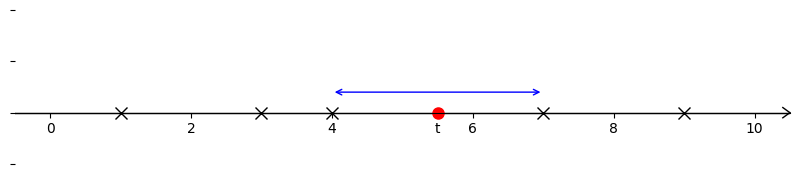
\includegraphics[width=\textwidth, keepaspectratio]{bus_arrival_timeline.png}
\end{figure}% --- CHUNK_METADATA_START ---
% src_checksum: e057243b85727e5b19906c356cf8a688eec87132c5e4aaa36c0c26d86a440531
% needs_review: True
% --- CHUNK_METADATA_END ---
\begin{itemize}
    \item \textbf{First reasoning:} Due to the memoryless property of the exponential distribution governing the inter-arrival times, my waiting time follows an $\text{Exp}(\lambda)$ distribution, with an average of $1/\lambda$.
    \item \textbf{Second reasoning:} I arrive randomly between two buses. By symmetry, the average waiting time would be half the typical interval length, i.e., $\frac{1}{2\lambda}$. This reasoning is incorrect.
\end{itemize}% --- CHUNK_METADATA_START ---
% src_checksum: 9a2a3bb3e6b8ebc791e545a1f4485064a81906dbd4ad831397708220ae0c6fd4
% needs_review: True
% --- CHUNK_METADATA_END ---
Let $S_n = Y_1 + \dots + Y_n$ be the arrival times of the buses. Let $k$ be such that $S_{k-1} < t \le S_k$. My waiting time is $S_k - t$. The error comes from the fact that the interval $[S_{k-1}, S_k]$ in which we "fall" is not a typical interval. There is a higher chance of falling into a large interval. Typically, this interval is twice as large as the average. The interval $Y_k = S_k - S_{k-1}$ does not follow the law $\text{Exp}(\lambda)$ because its distribution depends on $t$.
